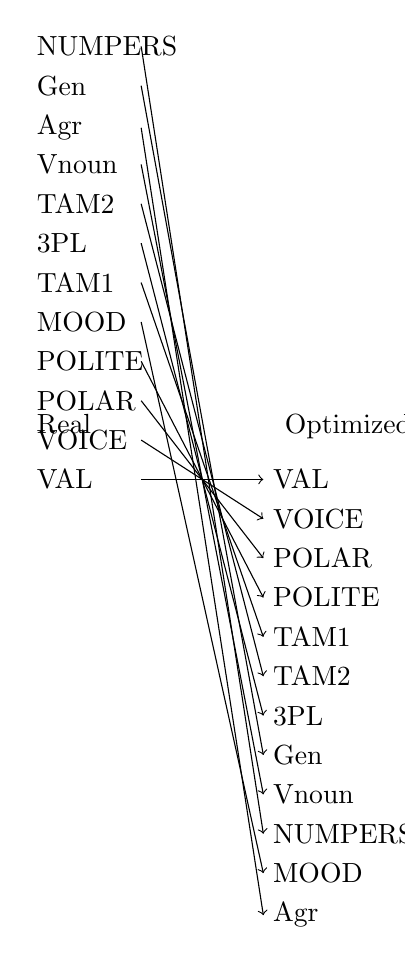
\begin{tikzpicture}[%
  % common options for blocks:
  block/.style = {draw, fill=blue!30, align=center, anchor=west,
              minimum height=0.65cm, inner sep=0},
  % common options for the circles:
  ball/.style = {circle, draw, align=center, anchor=north, inner sep=0}]
  \node[rectangle,text width=1.2cm,anchor=base] (A0) at (1,-0.3) {Real};
  \node[rectangle,text width=0.9cm,anchor=base] (B0) at (4,-0.3) {Optimized};
\node[rectangle,text width=1.2cm,anchor=base] (A1) at (1,-1.0) {VAL};
\node[rectangle,text width=1.2cm,anchor=base] (A2) at (1,-0.5) {VOICE};
\node[rectangle,text width=1.2cm,anchor=base] (A3) at (1,0.0) {POLAR};
\node[rectangle,text width=1.2cm,anchor=base] (A4) at (1,0.5) {POLITE};
\node[rectangle,text width=1.2cm,anchor=base] (A5) at (1,1.0) {MOOD};
\node[rectangle,text width=1.2cm,anchor=base] (A6) at (1,1.5) {TAM1};
\node[rectangle,text width=1.2cm,anchor=base] (A7) at (1,2.0) {3PL};
\node[rectangle,text width=1.2cm,anchor=base] (A8) at (1,2.5) {TAM2};
\node[rectangle,text width=1.2cm,anchor=base] (A9) at (1,3.0) {Vnoun};
\node[rectangle,text width=1.2cm,anchor=base] (A10) at (1,3.5) {Agr};
\node[rectangle,text width=1.2cm,anchor=base] (A11) at (1,4.0) {Gen};
\node[rectangle,text width=1.2cm,anchor=base] (A12) at (1,4.5) {NUMPERS};
\node[rectangle,text width=1.2cm,anchor=base] (B1) at (4,-1.0) {VAL};
\node[rectangle,text width=1.2cm,anchor=base] (B2) at (4,-1.5) {VOICE};
\node[rectangle,text width=1.2cm,anchor=base] (B3) at (4,-2.0) {POLAR};
\node[rectangle,text width=1.2cm,anchor=base] (B4) at (4,-2.5) {POLITE};
\node[rectangle,text width=1.2cm,anchor=base] (B5) at (4,-3.0) {TAM1};
\node[rectangle,text width=1.2cm,anchor=base] (B6) at (4,-3.5) {TAM2};
\node[rectangle,text width=1.2cm,anchor=base] (B7) at (4,-4.0) {3PL};
\node[rectangle,text width=1.2cm,anchor=base] (B8) at (4,-4.5) {Gen};
\node[rectangle,text width=1.2cm,anchor=base] (B9) at (4,-5.0) {Vnoun};
\node[rectangle,text width=1.2cm,anchor=base] (B10) at (4,-5.5) {NUMPERS};
\node[rectangle,text width=1.2cm,anchor=base] (B11) at (4,-6.0) {MOOD};
\node[rectangle,text width=1.2cm,anchor=base] (B12) at (4,-6.5) {Agr};
\draw[->] (A1.east) to (B1.west);
\draw[->] (A2.east) to (B2.west);
\draw[->] (A3.east) to (B3.west);
\draw[->] (A4.east) to (B4.west);
\draw[->] (A5.east) to (B11.west);
\draw[->] (A6.east) to (B5.west);
\draw[->] (A7.east) to (B7.west);
\draw[->] (A8.east) to (B6.west);
\draw[->] (A9.east) to (B9.west);
\draw[->] (A10.east) to (B12.west);
\draw[->] (A11.east) to (B8.west);
\draw[->] (A12.east) to (B10.west);
\end{tikzpicture}